\documentclass[../../Problems]{subfiles}
\begin{document}
\subsection{Gauss Circle Problem}\label{pp:gausscircle}
Consider a circle in the $x-y$ plane with center at the origin and radius $r\geq 0$ ($r\in\mathbb{R}$ such that $r^2=n\in\mathbb{Z}$).\\
Gauss's circle problem asks the number of lattice points $N(r)$ in the interior or on the circumference of this circle.\\
These points are of the form $(x,y) \in \mathbb{Z}^2$ such that $x^2+y^2\leq r^2=n$. Also, note that $N(r)\sim\pi r^2$ (why?).
\begin{figure}[H]
\centering
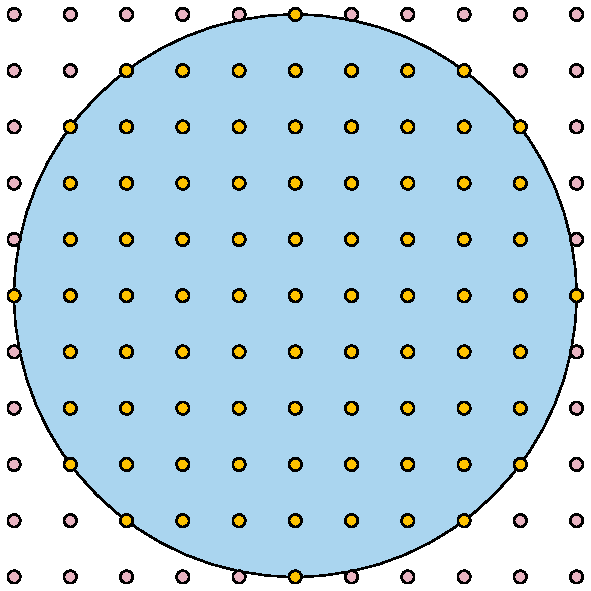
\includegraphics[width = 0.2\linewidth]{Gauss Circle Problem.pdf}
\caption{A circle with $r=5$ units bounding 81 integer points. $N(r) = 81 \sim\pi r^2\approx78.54$}
\end{figure}
% \begin{SCfigure}
% \centering
% 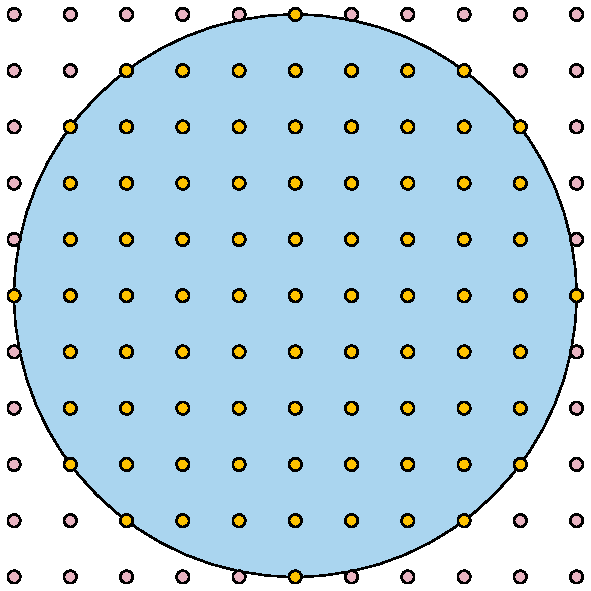
\includegraphics[width = 0.2\linewidth]{Gauss Circle Problem.pdf}
% \caption{A circle with $r=5$ units bounding 81 integer points. $N(r) = 81 \sim\pi r^2\approx78.54$}
% \end{SCfigure}
\vspace*{-1em}
Consider the subproblem of finding $M(i)$ -- the number of $(x,y) \in \mathbb{Z}^2$ such that $x^2+y^2=i$ where $i\in\{;0,1,\ldots,n\}.$ %$0\leq i\leq r^2=n$.
\\Clearly $\displaystyle N(r)=\sum_{i=0}^{r^2} M(i) \rightarrow N(\sqrt{n})=\sum_{i=0}^{n} M(i)$. Now,\vspace*{-1em}
\begin{equation}
	M(i) = 4\sum_{j|n}\chi(j)\quad\text{where}\quad\chi(n)=\begin{cases} 
      1 & \text{if $n\%4=1$}\\
      -1 & \text{if $n\%4=3$}\\
      0 & \text{else}
   \end{cases}
\end{equation}
\textbf{Problem Statement:}\\
Calculate $N(\sqrt{n})$ for a given $n$; i.e. the number of lattice points $(x,y)$ such that $x^2+y^2\leq n$.
\begin{testcasesFunction}
	{$t$ \hfill(number of test cases, an integer)\\
	$n_1\ n_2\ \ldots\ n_t$ \hfill($t$ space seperated integers for each testcase)}
	{$N(\sqrt{n_i})$ \hfill(each test case space seperated)}
	{$1 < n_i \leq 10^{7}$}
	{\texttt{int X(int n)} -- returns $\chi(n)$\\
	\texttt{int count\_lattice\_points(int n)} -- returns $M(n)$}
	{15\\0 1 2 3 5 10 20 30 50 100 1000 10000 100000 1000000 10000000}
	{1 5 9 9 21 37 69 97 161 317 3149 31417 314197 3141549 31416025}
	{https://github.com/paramrathour/CS-101/tree/main/Starter Codes/Gauss Circle Problem.cpp}
\end{testcasesFunction}
\begin{noteI}
Does the last few outputs look familiar? How can this happen? :o\\
Also, if the last output took a long time then think how you can do the calculations faster?
\end{noteI}
\begin{funvideo}
\href{https://youtu.be/NaL_Cb42WyY}{Pi hiding in prime regularities -- 3Blue1Brown}\\
\href{https://youtu.be/VftM4LpTrkI}{Your New Favorite Formula For Pi -- BriTheMathGuy}
\end{funvideo}
\end{document}